\documentclass{article}

\usepackage{times}
\usepackage{geometry}
\geometry{a4paper,left=0.6cm,right=0.7cm,top=2cm,bottom=1cm,columnsep=0.8cm}
\usepackage{fontawesome}
\usepackage[hidelinks]{hyperref}
\usepackage{multicol}
\usepackage{tikz}
\usepackage{hyphsubst}
\usepackage{moresize}
\usepackage{hyphenat}
\usepackage{tabularx}
\usepackage{xcolor}
\usepackage{enumitem}
\usetikzlibrary{calc, positioning}      
\newcolumntype{Y}{>{\RaggedRight\arraybackslash}X}

% Définition des couleurs
\definecolor{maincolor}{HTML}{f0fafc}
\definecolor{seccolor}{HTML}{ffffff}
\definecolor{gray}{HTML}{8c94a9}
\definecolor{sidetext}{HTML}{59cee5}

% Solution robuste pour la bande bleue sur toute la hauteur
\usepackage{eso-pic}
\AddToShipoutPictureBG{%
  \begin{tikzpicture}[remember picture,overlay]
    \fill[maincolor] 
        (current page.north west) rectangle 
        ([xshift=0.3\paperwidth] current page.south west);
  \end{tikzpicture}%
}

% Configuration des listes
\setlist[itemize]{itemsep=-2pt,topsep=0pt,leftmargin=1.08cm}
\renewcommand{\labelitemi}{\textcolor{sidetext}{\footnotesize$\bullet$}}

\setlength{\parindent}{0pt}
\usepackage{paracol}
\columnratio{0.3}

\begin{document}

\pagestyle{empty}

\begin{paracol}{2}
% ------------------------------------------------------------------
% Colonne gauche - Section personnelle
% ------------------------------------------------------------------
\color{sidetext}
\begin{center}
    \begin{tikzpicture}
        \clip (0,0) circle (1.5cm) node[anchor=center] {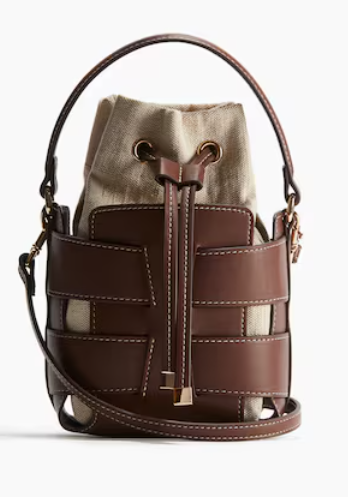
\includegraphics[width=3cm]{cb9b8964968c4865a601f7de0d7e4dee.png}}; 
    \end{tikzpicture}

    \vspace{5mm}
    
    {\color{black}\LARGE \textbf{Dora SARKIS}}
    
    \vspace{3mm}
    
    {\large{Gérante \& Directrice d’événementiel}}
\end{center}

{\color{gray}\rule{\linewidth}{0.4pt}} \\

% ------------------ Coordonnées -------------------
\begin{tabular}{@{}c l}
    \faPhone{} & 
    \begin{tabular}[t]{@{}l@{}}
        {\color{gray}Téléphone} \\
        06\,90\,59\,69\,69
    \end{tabular} \\
    \\
    \faMapMarker{} & 
    \begin{tabular}[t]{@{}l@{}}
        {\color{gray}Adresse} \\
        53 résidence Les Citronnelles
    \end{tabular} \\
    \\
    \faEnvelope{} & 
    \begin{tabular}[t]{@{}l@{}}
        {\color{gray}Mail} \\
        leroyalriviera@gmail.com
    \end{tabular} \\
\end{tabular}

{\color{gray}\rule{\linewidth}{0.4pt}} \\

% ------------------ Compétences -------------------
\vspace{3mm}
{\color{black}{Compétences Clés}}

\vspace{5mm}

\begin{tabular}{@{}c l}
    \textcolor{sidetext}{\faBriefcase} & Gestion d’entreprise \\
    \\
    \textcolor{sidetext}{\faHandshakeO} & Négociation commerciale \\
    \\
    \textcolor{sidetext}{\faUsers} & Relation client \\
    \\
    \textcolor{sidetext}{\faCalendarCheckO} & Organisation d’événements \\
    \\
    \textcolor{sidetext}{\faLineChart} & Management \& gestion administrative \\
    \\
    \textcolor{sidetext}{\faGavel} & Intérêt pour le droit commercial, des affaires et immobilier \\
\end{tabular}

% Espace flexible pour étendre la colonne gauche
\vfill
~

\switchcolumn
% ------------------------------------------------------------------
% Colonne droite - Contenu professionnel
% ------------------------------------------------------------------
\color{black}

% ------------------ Profil ------------------------
\textcolor{black}{\Large \textbf{Profil Professionnel}} \\

Entrepreneure passionnée totalisant plus de 15 ans d’expérience dans le commerce de détail, l’événementiel et la gestion de structures culturelles. Habituée à piloter des équipes, négocier avec des partenaires variés et orchestrer des projets de A à Z. Spécialisée dans la création d’offres sur-mesure pour la clientèle mariage ainsi que dans l’exploitation de locaux commerciaux. Rigueur, autonomie et sens aigu du service client guident chacune de ses missions.\\[8pt]

% ------------------ Expérience --------------------
\textcolor{black}{\Large \textbf{Expérience Professionnelle}} \\

% Expérience 1 ------------------------------------------------------
\colorbox{maincolor}{%
  \begin{minipage}{\linewidth}
    \begin{tabular}{@{}l l r}
        \textcolor{sidetext}{\faBriefcase} & 
        \textbf{Gérante – Boutique \& Locaux commerciaux} &  
        \footnotesize{2019 -- Présent} \\
        & \textit{Pointe-à-Pitre} & \\
    \end{tabular}
    \begin{itemize}
        \item Supervision d’une boutique et gestion locative de plusieurs espaces commerciaux. 
        \item Pilotage complet des opérations : approvisionnements, relation fournisseurs, administration et comptabilité. 
        \item Développement de la clientèle par une négociation active et un service personnalisé.
    \end{itemize}
  \end{minipage}%
}

\vspace{5mm}

% Expérience 2 ------------------------------------------------------
\colorbox{maincolor}{%
  \begin{minipage}{\linewidth}
    \begin{tabular}{@{}l l r}
        \textcolor{sidetext}{\faBriefcase} & 
        \textbf{Directrice – Salle de spectacle} &  
        \footnotesize{2012 -- 2018} \\
        &  & \\
    \end{tabular}
    \begin{itemize}
        \item Management des équipes et organisation de la programmation événementielle. 
        \item Coordination logistique et budgétaire, suivi administratif et réglementaire. 
        \item Promotion des spectacles et négociation avec artistes, prestataires et partenaires.
    \end{itemize}
  \end{minipage}%
}

\vspace{5mm}

% Expérience 3 ------------------------------------------------------
\colorbox{maincolor}{%
  \begin{minipage}{\linewidth}
    \begin{tabular}{@{}l l r}
        \textcolor{sidetext}{\faBriefcase} & 
        \textbf{Gérante fondatrice – Joykiss} &  
        \footnotesize{2008} \\
        &  & \\
    \end{tabular}
    \begin{itemize}
        \item Création d’une boutique dédiée au mariage, incluant services de wedding planning et design. 
        \item Gestion quotidienne, négociations fournisseurs et développement d’une offre sur-mesure. 
        \item Accompagnement client de la conception à la réalisation de l’événement.
    \end{itemize}
  \end{minipage}%
}

\vspace{8mm}

% ------------------ Formation ---------------------
\textcolor{black}{\Large \textbf{Formation}} \\

% Diplôme 1 ---------------------------------------------------------
\begin{tabular}{@{}c l}
    \textcolor{sidetext}{\faGraduationCap} & 
    \begin{tabular}[t]{@{}l@{}}
        \textbf{Formation en décoration événementielle} \\
        Centre ABC \\
        2008 \\
        Cette formation a permis d’acquérir les bases créatives et techniques pour concevoir des décors sur-mesure lors d’événements.
    \end{tabular} \\
\end{tabular}

\vspace{5mm}

% Diplôme 2 ---------------------------------------------------------
\begin{tabular}{@{}c l}
    \textcolor{sidetext}{\faGraduationCap} & 
    \begin{tabular}[t]{@{}l@{}}
        \textbf{BTS Commerce international (inachevé)} \\
        CNED \\
        2008 \\
        Approfondissement des pratiques d’import-export et des négociations commerciales à l’échelle internationale.
    \end{tabular} \\
\end{tabular}

\vspace{5mm}

% Diplôme 3 ---------------------------------------------------------
\begin{tabular}{@{}c l}
    \textcolor{sidetext}{\faGraduationCap} & 
    \begin{tabular}[t]{@{}l@{}}
        \textbf{Baccalauréat professionnel Commerce} \\
        CNED \\
        2006 \\
        Formation axée sur la vente, la relation client et les techniques de gestion commerciale.
    \end{tabular} \\
\end{tabular}

\vspace{8mm}
\end{paracol}

\end{document}